\documentclass[11pt,a4paper]{ctexart}
\usepackage{amsmath,amssymb,amsthm}
\usepackage{graphicx}
\title{\vspace{-5ex}}
\author{基科32 曾柯又 2013012266}
\date{\vspace{-5ex}}
\linespread{1.8}
\begin{document}
\maketitle
\paragraph{1}
(a)A,B的选择分别为(0,1),(0,2),(0,3),(1,2),(1,3)时,A胜利,故A胜利的概率为$\frac{5}{8}$\\
(b)第三次冲突后,A选择0,1,B选择1,...7。可以计算出A再次胜利的几率是$\frac{13}{16}$\\
(c)A第n次获胜的概率是$ 1 - \frac{3}{2^{n+1}}$,当$n \geq 10 $时,B的选择区间固定在$0\sim1023$,A获胜的概率为$1 - \frac{3}{2^{11}}$,当$n > 16$时,B不再尝试,A获胜的概率为1,将所有概率乘起来,可以得到,A赢得所有竞争的概率为$\prod_{n = 2}^{10}(1 - \frac{3}{2^{n+1}})\times(1 - \frac{3}{2^{11}})^6 \approx 0.415$\\
(d)A,B的选择分别为(1,0)时,B获胜,故B胜利的概率为$\frac{1}{8}$
(e)和(c)类似,可以计算得B全部获胜的概率为$0.052$。
\paragraph{2}
如图给端口编号\\
\graphicspath{ {/home/cengq/Documents/homework} }
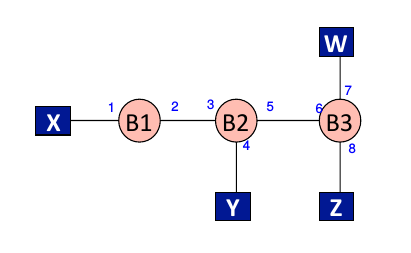
\includegraphics[scale=0.5]{p.png}\\
(a)B1,B2,B3都收到该帧并转发,1,3,6端口都将有X记录。\\
(b)B1,B2,B3都收到该帧并转发,2,5,8端口都将有Z记录。\\
(c)B1,B2受到帧并转发,B3未收到,2,4端口有Y记录。\\
(d)B3,B2受到帧并转发,B1未收到,转发表不会发生变化。\\
若节点W开始就运行tcpdump,则能收到(a),(d)时间的数据帧。
\end{document}